\documentclass[11pt]{article}
%\documentclass{book}
\usepackage[utf8]{inputenc}
\usepackage[T1]{fontenc}
\usepackage[french]{babel}
\usepackage[top=1.8cm, bottom=1.8cm, left=1.8cm, right=1.8cm]{geometry}
\usepackage[linktocpage,colorlinks=false]{hyperref}
\usepackage{graphicx}
\usepackage{epsfig}
\usepackage{amssymb}
\usepackage{amsmath}
\usepackage{array}
\usepackage{subfig}
\usepackage{multicol}
\usepackage{caption}
\usepackage{algorithm}
\usepackage{color}
\usepackage{algorithmic}
\hypersetup{
    colorlinks=true,
    breaklinks=true,
    urlcolor=red,
}
\parskip=5pt

\title{\huge{\textbf Calcul sécurisé - Attaque par faute sur DES}}
\author{CAUMES Clément 21501810}
\date{Master 1 Informatique SeCReTs}

\begin{document}

\maketitle
\vspace{20em}
%\begin{center}\includegraphics{pictures/Application.png}\end{center}
\newpage

\tableofcontents
\newpage

\section{Question 1 : Attaque par faute sur le DES}

Une attaque par faute consiste à changer le résultat d'un sous calcul afin d'obtenir une information secrète. Ce changement va donc produire volontairement une erreur. Cette attaque est physique car, pour modifier la valeur de certains bits, il est nécessaire d'agir physiquement sur les composants électroniques. 
Dans le cas du DES avec une attaque par faute sur la valeur de sortie $R_{15}$ du $15^{e}$ tour, cela signifie que la valeur $R_{15}$ va être changer par l'attaquant. 

\begin{center}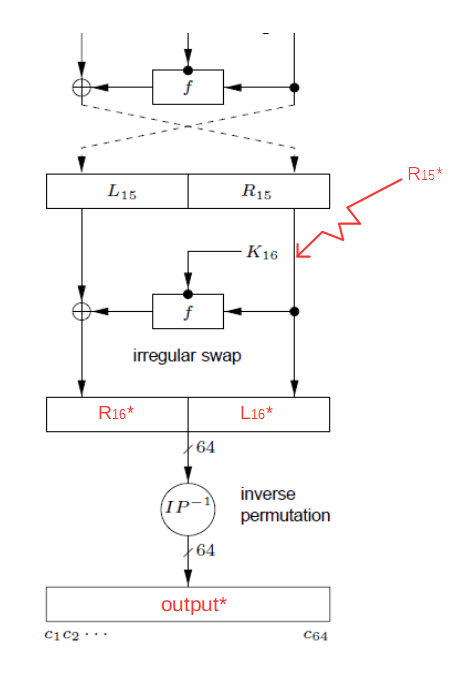
\includegraphics[scale=0.6]{../pictures/fauteR15.png}\end{center}

A partir de cette attaque, il est possible de retrouver la clé secrète utilisée par la victime à partir de la sous clé $K_{15}$. On suppose ici que nous sommes l'attaquant et que nous avons réussi à obtenir de la victime le message clair associé à son message chiffrée (avec une clé inconnue pour le moment, qui est à trouver). De plus, nous avons eu de la victime 32 chiffrés (toujours avec la même clé) et dont on a réussi à faire une attaque par faute. 

\section{Question 2 : Application concrète}

1. Cette attaque par faute sur le dernier tour du DES comporte plusieurs étapes : 

\begin{itemize}
	\item étape 1 : trouver $R_{15}$ à partir du chiffré juste et les $R_{15}*$ à partir des chiffrés faux. \newline Pour cela, on fait une permutation initiale (qui annule la permutation finale $IP^{-1}$) pour trouver $L_{16}$ et $R_{16}$. On fera de même pour $R_{15}*$ à partir des chiffrés faux. On peut désormais écrire les formules suivantes : \newline \newline $R_{16}= L_{15} \oplus f(K_{16}, R_{15})$ et $L_{16}=R_{15}$ pour le chiffré juste. 
	\newline $R_{16}*= L_{15} \oplus f(K_{16}, R_{15}*)$ et $L_{16}*=R_{15}*$ pour les chiffrés faux. \newline \newline Le but ici est d'obtenir $K_{16}$ : pour cela, on fait le XOR entre $R_{16}$ et un $R_{16}*$. Ce qui nous donne l'équation suivante : \newline \newline
	$R_{16} \oplus R_{16}* =  L_{15} \oplus f(K_{16}, R_{15}) \oplus L_{15} \oplus f(K_{16}, R_{15}*)$ \newline 
	%\newline \Leftrightarrow g$
	Les $L_{15}$ s'annulent et on obtient : $R_{16} \oplus R_{16}* = f(K_{16}, R_{15}) \oplus f(K_{16}, R_{15}*)$ \newline \newline
	Or, $f(K_{i+1}, R_{i})=P(S(E(R_{i})\oplus K_{i+1})) = P(S_1(E(R_i)\oplus K_{i+1})_{b_1\to b_6} || ... || S_8(E(R_i)\oplus K_{i+1})_{b_{43}\to b_{48}})$ \newline
		
	\item étape 2 : pour chaque chiffré faux (associé à son $R_{15}*$), établir 8 équations pour chaque boîte-S. \newline
	
	$P^{-1}(R_{16}\oplus R_{16}*)_{b_1\to b_4} = S_1(E(R_{15})\oplus K_{16})_{b_1\to b_4} \oplus S_1(E(R_{15}*)\oplus K_{16})_{b_1\to b_4}$
	
	$P^{-1}(R_{16}\oplus R_{16}*)_{b_5\to b_{8}} = S_2(E(R_{15})\oplus K_{16})_{b_5\to b_{8}} \oplus S_2(E(R_{15}*)\oplus K_{16})_{b_5\to b_{8}}$
	
	$P^{-1}(R_{16}\oplus R_{16}*)_{b_{9}\to b_{12}} = S_3(E(R_{15})\oplus K_{16})_{b_{9}\to b_{12}} \oplus S_3(E(R_{15}*)\oplus K_{16})_{b_{9}\to b_{12}}$
	
	$P^{-1}(R_{16}\oplus R_{16}*)_{b_{13}\to b_{16}} = S_4(E(R_{15})\oplus K_{16})_{b_{13}\to b_{16}} \oplus S_4(E(R_{15}*)\oplus K_{16})_{b_{13}\to b_{16}}$
			
	$P^{-1}(R_{16}\oplus R_{16}*)_{b_{17}\to b_{20}} = S_5(E(R_{15})\oplus K_{16})_{b_{17}\to b_{20}} \oplus S_5(E(R_{15}*)\oplus K_{16})_{b_{17}\to b_{20}}$
				
	$P^{-1}(R_{16}\oplus R_{16}*)_{b_{21}\to b_{24}} = S_6(E(R_{15})\oplus K_{16})_{b_{21}\to b_{24}} \oplus S_6(E(R_{15}*)\oplus K_{16})_{b_{21}\to b_{24}}$
					
	$P^{-1}(R_{16}\oplus R_{16}*)_{b_{25}\to b_{28}} = S_7(E(R_{15})\oplus K_{16})_{b_{25}\to b_{28}} \oplus S_7(E(R_{15}*)\oplus K_{16})_{b_{25}\to b_{28}}$
						
	$P^{-1}(R_{16}\oplus R_{16}*)_{b_{29}\to b_{32}} = S_8(E(R_{15})\oplus K_{16})_{b_{29}\to b_{32}} \oplus S_8(E(R_{15}*)\oplus K_{16})_{b_{29}\to b_{32}}$ \newline
	
	\item étape 3 : éliminer les équations dont $P^{-1}(R_{16}\oplus R_{16}*)_{b_x\to b_y}$ s'annulent.
	[ATTENTION SI SX() XOR SX() vaut 0 aussi] \newline
	
	\item étape 4 : faire une attaque exhaustive sur les sorties de chaque boîte-S. Cela permettra d'obtenir plusieurs cas possibles pour les entrées de celle-ci. En effet, il y a plusieurs solutions possibles pour la sortie d'une boîte-S, sachant qu'elles ne sont pas linéaires. De ce fait, on récupère toutes les solutions possibles pour chaque boîte-S. Une solution commune sera présente pour chaque chiffré faux qui sera la portion de bits de $K_{16}$. 
	

\end{itemize}

\section{Question 3 : Retrouver la clé complète du DES}

1. Dans la question précédente, nous avons réussi à obtenir la clé secrète $K_{16}$ qui contient 48 bits. En analysant le schéma de création des 16 sous-clés (de 48 bits) à partir de la clé secrète (de 56 bits), on peut en déduire la clé secrète. Cela comporte plusieurs étapes : 

\begin{center}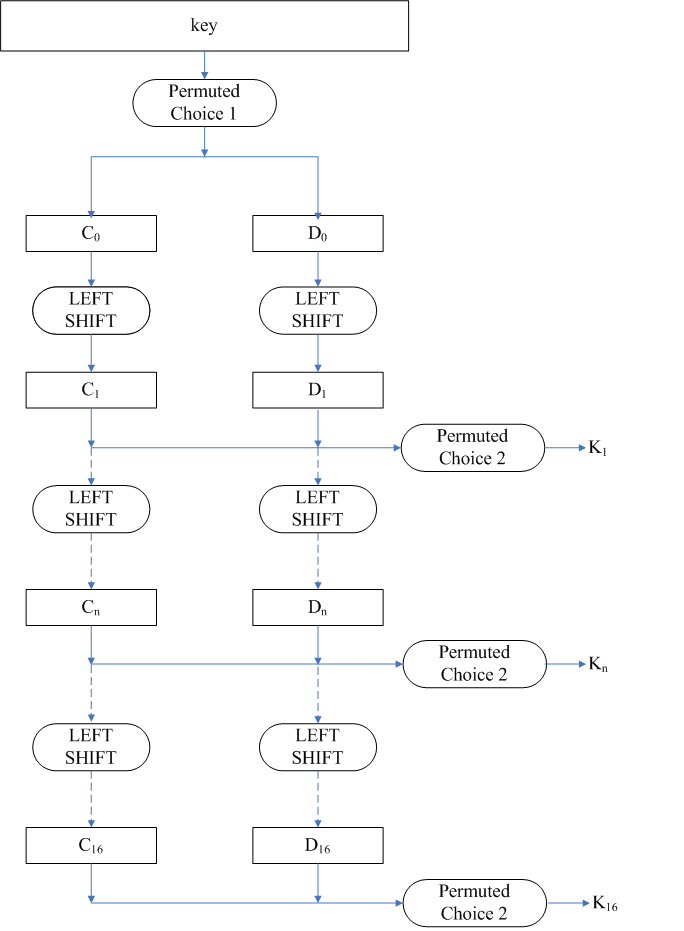
\includegraphics[scale=0.3]{../pictures/key_schedule.png}\end{center}

\begin{itemize}
	\item étape 1 : effectuer une permutation inverse $PC_{2}^{-1}(K_{16})$ afin d'obtenir $C_{16}$ et $D_{16}$.
	Il est important de noter que lors de cette permutation inverse, 8 bits sont inconnus. En effet, on passe de $48$ bits à $2 \times 28 = 56$ bits. Il y a donc 8 bits qu'on ne peut déduire à partir de $K_{16}$. \newline
	
	\begin{center}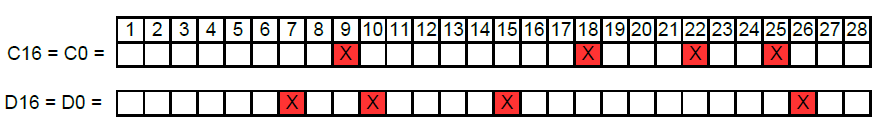
\includegraphics[scale=0.4]{../pictures/C0_D0.png}\end{center}
	
	Sur ce schéma, les bits encore inconnus sont marqués par "X". \newline
	
	
	\item étape 2 : Déduire $C_{0}$ et $D_{0}$ à partir de $C_{16}$ et $D_{16}$. En effet, $C_{0}=C_{16}$ et $D_{0}=D_{16}$ puisque la somme des shifts circulaires donne $28$ qui correspond à la taille des blocs $C_i$ et $D_i$. Les 8 bits inconnus n'ont donc pas bougé de place dans $C_0$ et $D_0$. \newline
	
	\item étape 3 : Effectuer une permutation inverse $PC_{1}^{-1}(C_{0}||D_{0})$ afin d'obtenir la clé finale sur 64 bits. On peut noter ici que les 8 bits inconnus sont mélangés dans la clé finale. De plus, 8 bits supplémentaires ont été rajoutés correspondant aux bits de parité. On a donc une clé finale sur 64 bits dont 16 bits sont inconnus. \newline
	
	\begin{center}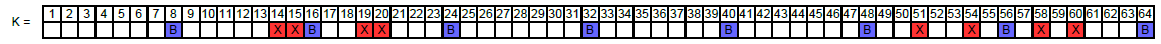
\includegraphics[scale=0.5]{../pictures/K64.png}\end{center}
	
	Sur le schéma ci-dessous, "B" correspond aux bits de parité. \newline
	
	\item étape 4 : Retrouver les 8 bits inconnus par une recherche exhaustive : $2^{8}=256$ cas possibles. Pour chaque clé possible, on faire le chiffrement DES avec en entrée la clé possible et le message clair fourni. Si la clé testée est celle recherchée, alors le chiffré obtenu sera identique à celui du chiffré correct fourni. \newline
	
	\item étape 5 : déduire les 8 bits de parité en s'assurant que chaque octet possède un nombre impair de bits à 1. 
	
	
\end{itemize}

2. On va effectuer les différentes étapes en détaillant : 

\begin{itemize}

\item On a obtenu précédemment lors de la recherche de la sous clé : $K_{16}= $ $02$ $10$ $B1$ $2C$ $47$ $79$. \newline \newline
Avec l'étape 1 et 2, on obtient : \newline 
- $C_{0}=C_{16}=$ $0110$ $00100100$ $00010000$ $00000100= 6241004$ \newline 
- $D_{0}=D_{16}=$ $0011$ $00000010$ $01001110$ $11001011= 3024ECB$ \newline
- $C_{0}||D_{0}=$ $62$ $41$ $00$ $43$ $02$ $4E$ $CB$ \newline
Les 8 bits inconnus à chercher sont à $0$. \newline

\item Avec l'étape 3, on obtient la clé DES sur 64 bits avec les 8 bits inconnus à 0 et les bits de parité également à 0 : \newline
- $K_{64}*=$ $50$ $90$ $0C$ $18$ $02$ $8E$ $D8$ $08$ \newline

\item On réalise l'attaque exhaustive et on trouve la solution en ajustant également les bits de parité et on obtient la solution finale de la clé DES sur 64 bits en hexadécimal: \newline 
\color{red}
$K_{64}=51$ $92$ $2C$ $19$ $02$ $8F$ $FD$ $49$
\color{black}



\end{itemize}


\end{document}